\documentclass{article}

\usepackage{graphicx}
\usepackage{tikz}
\usepackage{tikzsymbols}
\usetikzlibrary{calc,patterns,shapes.geometric}
\pagestyle{empty}
\usepackage[margin=0pt]{geometry}
\geometry{papersize={14in,12in}}

\def\centerarc[#1](#2)(#3:#4:#5){\draw[#1] ($(#2)+({#5*cos(#3)},{#5*sin(#3)})$) arc (#3:#4:#5);}

\begin{document}
	\begin{figure}
		\centering
		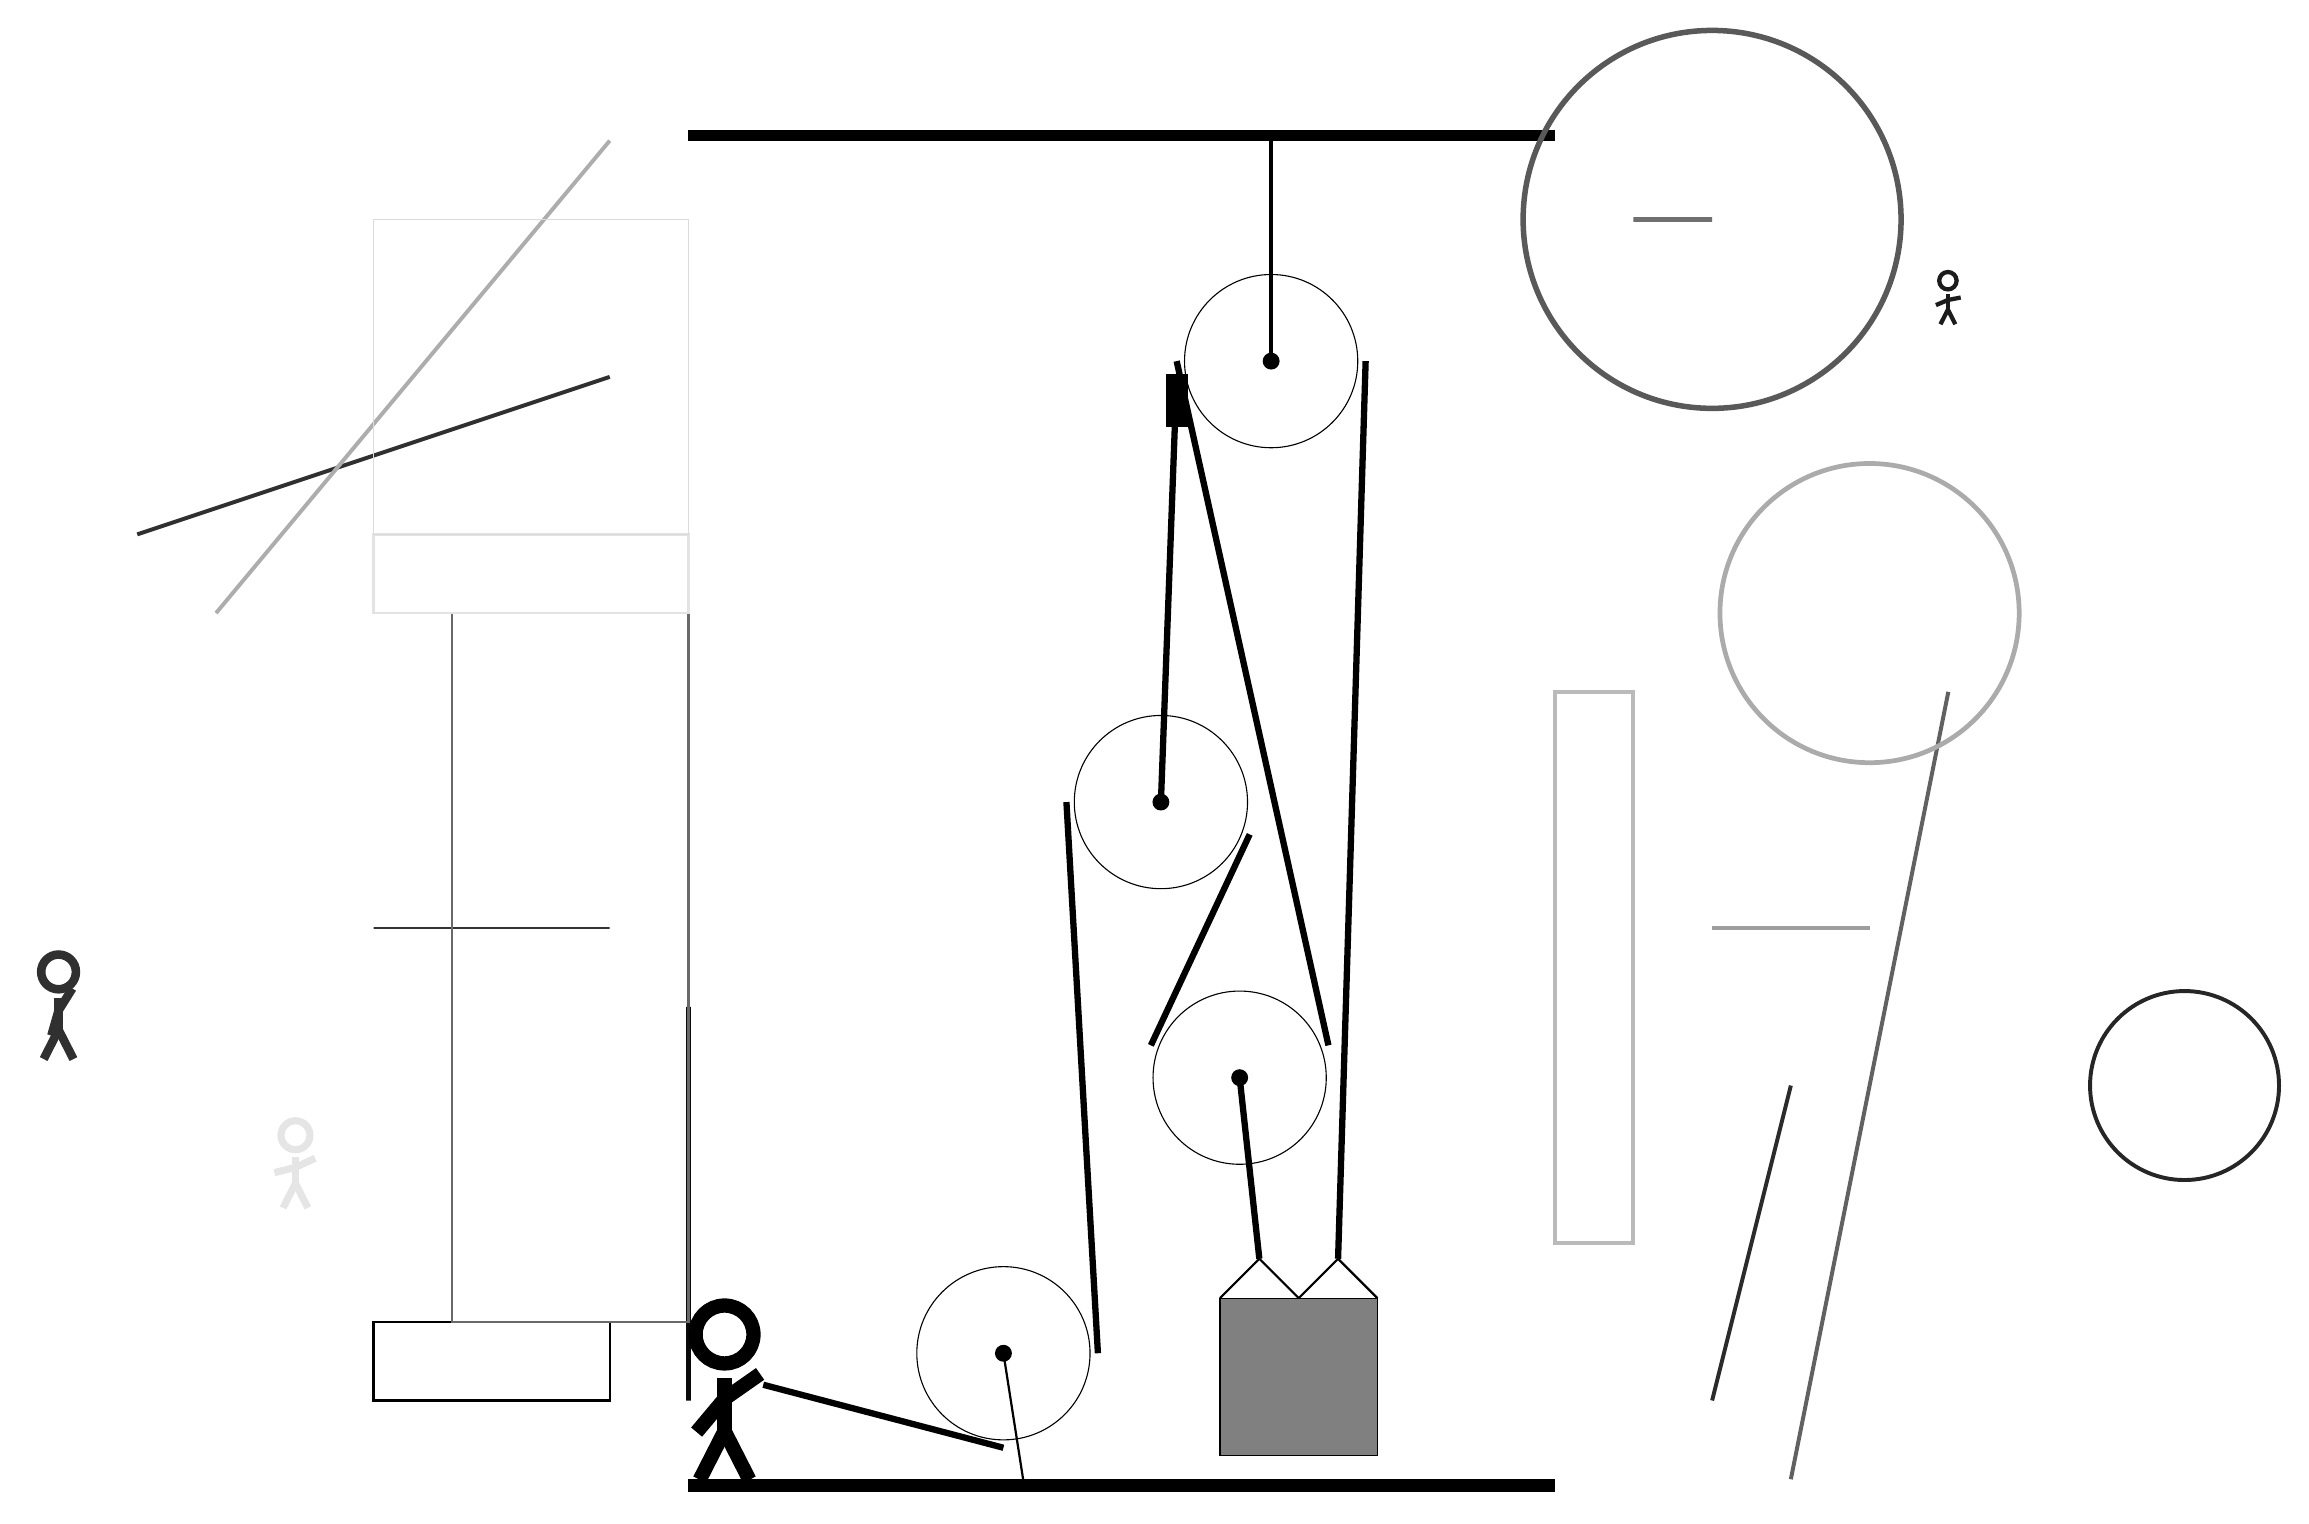
\begin{tikzpicture}
			%%%%% START %%%%%
			
			\draw[fill=black] (-6, 14) rectangle (5, 14.125);
			
			\draw (0, 5.6) circle (1.1);
			\draw[fill=black] (0, 5.6) circle (0.1);
			
			\draw (1, 2.1) circle (1.1);
			\draw[fill=black] (1, 2.1) circle (0.1);
			
			\draw (1.4, 11.2) circle (1.1);
			\draw[fill=black] (1.4, 11.2) circle (0.1);
			\draw[very thick] (1.4, 11.2) -- (1.4, 14);
			
			\draw (-2, -1.4) circle (1.1);
			\draw[fill=black] (-2, -1.4) circle (0.1);
			\draw[thick] (-2, -1.4) -- (-1.75, -3);
			
			\draw[line width=0.3mm, color=black!100] (-7, -2) rectangle (-10, -1);
			
			\node[line width=0.5mm, color=black!10] at (-11, 1) {\Strichmaxerl[5][14][25]};
			\draw[line width=0.7mm, color=black!56] (6, 13) rectangle (7, 13);
			\draw [line width=0.6mm, color=black!94](9, 10) circle (0.0);
			
			\node[line width=0.2mm, color=black!89] at (10, 12) {\Strichmaxerl[3][23][11]};
			\draw[line width=0.5mm, color=black!62](8, -3) -- (10, 7);
			
			\draw[line width=0.5mm, color=black!81](-7, 11) -- (-13, 9);
			\draw[line width=0.5mm, color=black!32](-7, 14) -- (-12, 8);
			\draw[line width=0.2mm, color=black!18] (-8, 13) rectangle (-9, 13);
			\draw[line width=0.2mm, color=black!80] (-7, 4) rectangle (-10, 4);
			\draw[line width=0.5mm, color=black!83](7, -2) -- (8, 2);
			\draw [line width=0.5mm, color=black!85](13, 2) circle (1.2);
			\draw[line width=0.7mm, color=black!96] (-6, 3) rectangle (-6, -2);
			\draw[line width=0.5mm, color=black!27] (5, 0) rectangle (6, 7);
			\draw[line width=0.3mm, color=black!59] (-6, 8) rectangle (-9, -1);
			\draw [line width=0.7mm, color=black!65](7, 13) circle (2.4);
			
			\draw[line width=0.3mm, color=black!11] (-6, 8) rectangle (-10, 9);
			\draw [line width=0.6mm, color=black!33](9, 8) circle (1.9);
			\draw[line width=0.2mm, color=black!14] (-6, 13) rectangle (-10, 9);
			\draw[line width=0.5mm, color=black!38](7, 4) -- (9, 4);
			\node[line width=0.2mm, color=black!81] at (-14, 3) {\Strichmaxerl[6][74][58]};
			
			
			\draw[thick]  (0.75, -0.7) -- (1.25, -0.2) -- (1.75, -0.7) -- (2.25, -0.2) -- (2.75, -0.7);
			\draw[fill=black!50] (0.75, -0.7) rectangle (2.75, -2.7);
			\draw[line width=0.8mm] (-5.05, -1.8) -- (-2, -2.6);
			\centerarc[line width=0.8mm](-2, -1.4)(270:360:1.2000000000000002);
			\draw[line width=0.8mm] (-0.8, -1.4) -- (-1.2, 5.6);
			\draw[line width=0.8mm] (0, 5.6) -- (0.2, 11.0);
			\draw[line width=0.8mm, fill=black](0.1, 10.4) rectangle (0.3, 11.0);
			\centerarc[line width=0.8mm](0, 5.6)(-20:180:1.2000000000000002);
			\draw[line width=0.8mm] (1.1276, 5.1896) -- (-0.1276, 2.5104);
			\centerarc[line width=0.8mm](1, 2.1)(160:380:1.2000000000000002);
			\draw[line width=0.8mm] (2.1276, 2.5104) -- (0.2, 11.2);
			\draw[line width=0.8mm](1, 2.1) -- (1.25, -0.2);
			\centerarc[line width=0.8mm](1.4, 11.2)(0:180:1.2000000000000002);
			\draw[line width=0.8mm] (2.6, 11.2) -- (2.25, -0.2);
			
			\node at (-5.5, -1.9) {\Strichmaxerl[10][50][35]};
			
			\draw[fill=black] (-6, -3) rectangle (5, -3.15);
			
			%%%%% END %%%%%
		\end{tikzpicture}
	\end{figure}	
\end{document}